\chapter{Marco Conceptual}


\section{Base de Datos} 	
\setlength{\parskip}{5mm}
Una base de datos (cuya abreviatura es BD) es una entidad en la cual se pueden almacenar datos de manera estructurada, con la menor redundancia posible. Diferentes programas y diferentes usuarios deben poder utilizar estos datos. Por lo tanto, el concepto de base de datos generalmente está relacionado con el de red ya que se debe poder compartir esta información. De allí el término base. Sistema de información es el término general utilizado para la estructura global que incluye todos los mecanismos para compartir datos que se han instalado. (\citet{bdbib}, 2016) 


\setlength{\parskip}{0mm}



\subsection{Sistema Manejador de Base de Datos}
\setlength{\parskip}{5mm}
Un sistema manejador de bases de datos (SGBD, por sus siglas en inglés) o DataBase Management System (DBMS) es una colección de software muy específico, cuya función es servir de interfaz entre la base de datos, el usuario y las distintas aplicaciones utilizadas.

Como su propio nombre indica, el objetivo de los sistemas manejadores de base de datos es precisamente el de manejar un conjunto de datos para convertirlos en información relevante para la organización, ya sea a nivel operativo o estratégico.
 
Lo hace mediante una serie de rutinas de software para permitir su uso de una manera segura, sencilla y ordenada. Se trata, en suma, de un conjunto de programas que realizan tareas de forma interrelacionada para facilitar la construcción y manipulación de bases de datos, adoptando la forma de interfaz entre éstas, las aplicaciones y los mismos usuarios. (\citet{smdbbib}, 2015)

El SMDB puede dividirse en tres subsistemas:
\setlength{\parskip}{0mm}
\begin{itemize}

    \item El sistema de administración de archivos: para almacenar información en un medio físico
    
    \item El DBMS interno: para ubicar la información en orden
    
    \item El DBMS externo: representa la interfaz del usuario

\end{itemize}



\setlength{\parskip}{5mm}
A continuación se presentarán algunos ejemplos de SMBD.
\setlength{\parskip}{0mm}

\subsection {PostgresSQL}
\setlength{\parskip}{5mm}
PostgreSQL es un sistema de gestión de bases de datos objeto-relacional, distribuido bajo licencia BSD y con su código fuente disponible libremente. Es el sistema de gestión de bases de datos de código abierto más potente del mercado.

PostgreSQL utiliza un modelo cliente/servidor y usa multiprocesos en vez de multihilos para garantizar la estabilidad del sistema. Un fallo en uno de los procesos no afectará el resto y el sistema continuará funcionando.

Sus características técnicas la hacen una de las bases de datos más potentes y robustas del mercado. Su desarrollo comenzo hace más de 16 años, y durante este tiempo, estabilidad, potencia, robustez, facilidad de administración e implementación de estándares han sido las características que más se han tenido en cuenta durante su desarrollo.

PostgreSQL funciona muy bien con grandes cantidades de datos y una alta concurrencia de usuarios accediendo a la vez a el sistema. (\citet{postgresbib}, 2011)
\setlength{\parskip}{0mm}


%\url{http://www.postgresql.org.es/sobre_postgresql}

\subsection{MySQL}
\setlength{\parskip}{5mm}
MySQL es un sistema de administración de bases de datos (Database Management System, DBMS) para bases de datos relacionales. Así, MySQL no es más que una aplicación que permite gestionar archivos llamados de bases de datos.

MySQL, como base de datos relacional, utiliza multiples tablas para almacenar y organizar la información. MySQL fue escrito en C y C++ y destaca por su gran adaptación a diferentes entornos de desarrollo, permitiendo su interactuación con los lenguajes de programación más utilizados como PHP, Perl y Java y su integración en distintos sistemas operativos.

También es muy destacable, la condición de open source de MySQL, que hace que su utilización sea gratuita e incluso se pueda modificar con total libertad, pudiendo descargar su código fuente. Esto ha favorecido muy positivamente en su desarrollo y continuas actualizaciones, para hacer de MySQL una de las herramientas más utilizadas por los programadores orientados a Internet.
\setlength{\parskip}{0mm}
(\citet{mysqlbib}, 2005)
%http://www.esepestudio.com/noticias/que-es-mysql

\subsection{Oracle}
\setlength{\parskip}{5mm}
Oracle la Primera Base de Datos Diseñada para Grid Computing, es un sistema de gestión de base de datos relacional fabricado por Oracle Corporation. Oracle es básicamente un herramienta cliente/servidor para la gestión de base de datos la gran potencia que tiene y su elevado precio hace que solo se vea en empresas muy grandes y multinacionales, por norma general. Oracle Corporation :es una de las mayores compañías de software del mundo. Sus productos van desde bases de datos (Oracle) hasta sistemas de gestión. Cuenta además, con herramientas propias de desarrollo para realizar potentes aplicaciones, como Oracle Designer

Desarrollado sobre Oracle Database, Oracle Content Database ha sido diseñada para que las organizaciones puedan controlar y gestionar grandes volúmenes de contenidos no estructurados en un único repositorio con el objetivo de reducir los costes y los riesgos asociados a la pérdida de información.
\setlength{\parskip}{0mm}
(\citet{oraclebib}, 2014) 

%https://iessanvicente.com/colaboraciones/oracle.pdf

\section{Base de datos móvil} 		

Es una Base de datos donde los usuarios pueden acceder a la información lejos de donde se encuentra almacenada la base de datos, se hace utilizando una conexión inalámbrica. (\citet{bdmovil}, 2012)

\subsection{Sistema manejador de base de datos móvil} 

\subsubsection{SQLite}
\setlength{\parskip}{5mm}


SQLite es una herramienta de software libre, que permite almacenar información en dispositivos empotrados de una forma sencilla, eficaz, potente, rápida y en equipos con pocas capacidades de hardware, como puede ser una PDA o un teléfono celular. SQLite implementa el estándar SQL92 y también agrega extensiones que facilitan su uso en cualquier ambiente de desarrollo. 

Esto permite que SQLite soporte desde las consultas más básicas hasta las más complejas del lenguaje SQL, y lo más importante es que se puede usar tanto en dispositivos móviles como en sistemas de escritorio, sin necesidad de realizar procesos complejos de importación y exportación de datos, ya que existe compatibilidad al 100\% entre las diversas plataformas disponibles, haciendo que la portabilidad entre dispositivos y plataformas sea transparente. (\citet{sqlitebib}, 2007)

Características:
\setlength{\parskip}{0mm}
\begin{itemize}

\item La base de datos completa se encuentra en un solo archivo.

\item Puede funcionar enteramente en memoria, lo que la hace muy rápida.

\item Tiene un footprint menor a 230KB.

\item Es totalmente autocontenida (sin dependencias externas).

\item Cuenta con librerías de acceso para muchos lenguajes de programación.

\item Soporta texto en formato UTF-8 y UTF-16, así como datos numéricos de 64 bits.

\item Soporta funciones SQL definidas por el usuario (UDF).

\item El código fuente es de dominio público y se encuentra muy bien documentado.

\end{itemize}


\subsubsection{SYBASE}
\setlength{\parskip}{5mm}
Es la abreviatura de "Adaptive Server Enterprise", el software de base de datos relacional fabricado y vendido por Sybase Inc. ASE es un software versátil, de clase empresarial RDBMS que es especialmente bueno en el manejo de cargas de trabajo OLTPASE, es utilizado de forma intensiva en el mundo financiero (bancos, bolsas de valores, compañías de seguros), en el comercio electrónico, así como en el área de prácticamente todos los demás. (\citet{sybasebib}, 2011)

Características:
\setlength{\parskip}{0mm}

\begin{itemize}

\item La opción IMD permite la virtualización y crecimiento de datos fundamental para satisfacer las necesidades de grandes volúmenes de datos y organizaciones con alta concurrencia de usuarios.

\item Permite a los clientes existentes de Sybase ASE adoptar fácilmente las nuevas características y optimizaciones sin la necesidad de una actualización de la base de datos

\item Copias de respaldo en línea y de alto rendimiento. 

\item Soporte a múltiples herramientas de desarrollo y lenguajes de programación, como PowerBuilder, Visual Basic, Java, PHP.

\item Técnicas de particionamiento semántico de tablas que aumentan la velocidad de acceso a los datos. 

\end{itemize}


\subsubsection{MICROSOFT SQL SERVER CE}
\setlength{\parskip}{5mm}

Microsoft SQL Server Compact en su actual versión 4.0 es una base de datos compacta para aplicaciones de escritorio y web. SQL Server Compact 4.0 posee un modelo de programación común a otras ediciones de SQL Server para el desarrollo tanto de aplicaciones nativas como administradas. SQL Server Compact ofrece funcionalidad de base de datos relacional en un espacio reducido: un sólido almacén de datos, un procesador de consultas de optimización y una conectividad confiable y escalable. (\citet{sqlservercebib}, 2016) 

Características:
\setlength{\parskip}{0mm}

\begin{itemize}

\item Integración con WebMatrix una pila de desarrollo web gratuita que integra un servidor web con marcos de trabajo de programación y base de datos.

\item SQL Server Compact 4.0 usa el algoritmo SHA2 para proteger los datos y proporcionar un alto nivel de seguridad. 

\item SqlServerCe está enfocado a funcionar sobre dispositivos con características limitadas

\item Posee un motor de base de datos así como un procesador y un optimizador de consultas especialmente diseñado para entornos móviles

\item Únicamente soporta tipos de datos de cadena compatibles con Unicode (nchar, nvarchar, ntext). 

\end{itemize}

(\citet{sqlserverce2bib}, 2016)

\subsection{Arquitectura de una base de datos móvil} 

%\begin{figure}[H]
%\begin{center}
%	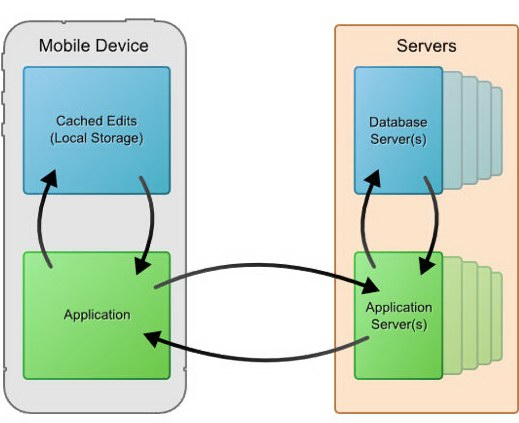
\includegraphics[width=13cm,height=8cm]{img/mobiledb.jpg}
%\end{center}
%\caption{Mobile divice. (Tomada de , 2014)}
%\label{fig:Mobiledb}
%\end{figure}



\section{Dispositivo móvil}
\setlength{\parskip}{5mm}
Dispositivo móvil (mobile device), también conocido como computadora de bolsillo o computadora de mano (palmtop o handheld), es un tipo de computadora de tamaño pequeño, con capacidades de procesamiento, con conexión a Internet, con memoria, diseñado específicamente para una función, pero que pueden llevar a cabo otras funciones más generales.

Estrictamente hablando, muchos de los llamados dispositivos móviles no tienen la capacidad de moverse. Más bien son dispositivos que pueden ser fácilmente transportados por sus usuarios
\setlength{\parskip}{0mm}

%Referecia
%↑ The University of California, Riverside, ed. (3 de diciembre de 2015). «When Apps Talk Behind Your Back» (en inglés). Consultado el 10 de diciembre de 2015. «We focused on a relatively neglected aspect of security research, which is the potential for good apps to leak personal information through the sites they interact with.»

\subsection{Tipos de dispositivos móviles}

\subsubsection{Teléfono Celular} 
\setlength{\parskip}{5mm}
Es un dispositivo inalámbrico electrónico que permite tener acceso a la red de telefonía celular o móvil. Se denomina celular debido a las antenas repetidoras que conforman la red, cada una de las cuales es una célula, si bien existen redes telefónicas móviles satelitales. Su principal característica es su portabilidad, que permite comunicarse desde casi cualquier lugar. Aunque su principal función es la comunicación de voz, como el teléfono convencional, su rápido desarrollo ha incorporado otras funciones como son cámara fotográfica, agenda, acceso a internet, reproducción de video e incluso GPS y reproductor mp3.

La comunicación telefónica es posible gracias a la interconexión entre centrales móviles y públicas. Según las bandas o frecuencias en las que opera el móvil, podrá funcionar en una parte u otra del mundo. La telefonía móvil consiste en la combinación de una red de estaciones transmisoras-receptoras de radio (repetidores, estaciones base o BTS) y una serie de centrales telefónicas de conmutación de 1.º y 5.º nivel (MSC y BSC respectivamente), que posibilita la comunicación entre terminales telefónicos portátiles (teléfonos móviles) o entre terminales portátiles y teléfonos de la red fija tradicional.
\setlength{\parskip}{0mm}
(\citet{celbib}, 2016)
%http://www.ecured.cu/Tel%C3%A9fono_celular

\subsubsection{Teléfonos Inteligentes}
\setlength{\parskip}{5mm}
Es un tipo de teléfono móvil construido sobre una plataforma informática móvil, con mayor capacidad de almacenar datos y realizar actividades, semejante a la de una minicomputadora, y con una mayor conectividad que un teléfono móvil convencional. El término «inteligente», que se utiliza con fines comerciales, hagan referencia a la capacidad de usarse como un computador de bolsillo, y llega incluso a reemplazar a una computadora personal en algunos casos.
(\citet{},2016)
\setlength{\parskip}{0mm}
\subsubsection{Tablets}
\setlength{\parskip}{5mm}
Es un dispositivo electrónico que tiene un tamaño intermedio entre el ordenador y el móvil. Sus características principales son las siguientes: su ligereza, su manejo intuitivo utilizando las manos, su elevada autonomía de uso y la no dependencia de otros accesorios complementarios.

Los sistemas operativos de estos dispositivos permiten una velocidad e inmediatez considerable, las aplicaciones que incorporan son muy accesibles y los procesos para su manejo son más rápidos que en los portátiles. Hay que tener presente que el tablet se maneja con las manos, probablemente la herramienta más dúctil y eficaz que existe (todavía las manos artificiales no han conseguido superar la destreza de las manos humanas).(\citet{tabletbib},2016)
\setlength{\parskip}{0mm}

%http://www.definicionabc.com/tecnologia/tablet.php


\section{Sistema Operativo Móvil}	
\setlength{\parskip}{5mm}
Un sistema operativo móvil o SO móvil es un sistema operativo que controla un dispositivo móvil al igual que los PCs que utilizan Windows o Linux, los dispositivos moviles tienen sus sistemas operativos como Android, IOS entre otros. Los sistemas operativos móviles son mucho más simples y están más orientados a la conectividad inalámbrica, los formatos multimedia para móviles y las diferentes maneras de introducir información en ellos.

Algunos de los sistemas operativos utilizados en los dispositivos móviles están basados en el modelo de capas.

\setlength{\parskip}{0mm}
\subsection{Tipos de sistemas operativos móviles}

\subsubsection{Android} 
\setlength{\parskip}{5mm}
Es un sistema operativo inicialmente pensado para teléfonos móviles, al igual que iOS, Symbian y Blackberry OS. Lo que lo hace diferente es que está basado en Linux, un núcleo de sistema operativo libre, gratuito y multiplataforma.

El sistema permite programar aplicaciones en una variación de Java llamada Dalvik. El sistema operativo proporciona todas las interfaces necesarias para desarrollar aplicaciones que accedan a las funciones del teléfono (como el GPS, las llamadas, la agenda, etc.) de una forma muy sencilla en un lenguaje de programación muy conocido como es Java
\setlength{\parskip}{0mm}
(\citet{androidbib}, 2016)
%t.xatakandroid.com/sistema-operativo/que-es-android

\subsubsection{iOS} 
\setlength{\parskip}{5mm}
Es un sistema operativo móvil desarrollado por Apple Inc. Inicialmente fue creado para el iPhone, pero con el tiempo fue adaptado para los demás dispositivos móviles de esta compañía (iPad y el iPod touch).

Este sistema operativo móvil está basado en el concepto de manipulación directa. Es decir, que el usuario puede interactuar directamente con la pantalla del dispositivo por medio de gestos multitáctiles como toques, pellizcos y deslices.
\setlength{\parskip}{0mm}
(\citet{iosbib}, 2016)


\subsubsection{Firefox OS}
\setlength{\parskip}{5mm}
Firefox OS (nombre clave: Boot to Gecko o B2G) es un sistema operativo móvil, basado en HTML5 con núcleo Linux, de código abierto para varias plataformas. Es desarrollado por Mozilla Corporation bajo el apoyo de otras empresas y una gran comunidad de voluntarios de todo el mundo. El sistema operativo está diseñado para permitir a las aplicaciones HTML5 comunicarse directamente con el hardware del dispositivo usando JavaScript y Open Web APIs.

Inicialmente estuvo enfocado en los dispositivos móviles, smartphones y tabletas, específicamente en el sector de gama baja, el 2 de julio de 2013, Telefónica comenzó la venta del primer terminal con Firefox OS, el ZTE Open.
\setlength{\parskip}{0mm}
(\citet{firefoxbib}, 2016)

%\section{Computación Móvil}	

%\subsection{Fases de la computación móvil}

%\subsection{Característica de la computación móvil}

\section{Aplicación Móvil}	

\subsection{Tipos de aplicaciones móviles}

\subsubsection{Aplicaciones Nativas}
\setlength{\parskip}{5mm}
Una aplicación nativa es la que se desarrolla de forma específica para un determinado  sistema operativo, llamado Software Development Kit o SDK. Cada una de las plataformas, Adroid, iOS o Windows Phone, tienen un sistema diferente, por lo que si quieres que tu app esté disponible en todas las plataformas se deberán de crear varias apps con el lenguaje del sistema operativo seleccionado.
Por ejemplo:
\setlength{\parskip}{0mm}
\begin{itemize}

	\item Las apps para iOS se desarrollan con lenguaje Objective-C
	
	\item Las apps para Android se desarrollan con lenguaje Java
	
	\item Las apps en Windows Phone se desarrollan en .Net

	
\end{itemize}
\setlength{\parskip}{5mm}
Cuando hablamos de desarrollo móvil casi siempre nos estamos refiriendo a aplicaciones nativas. La principal ventaja con respecto a los otros dos tipos, es la posibilidad de acceder a todas las características del hardware del móvil: cámara, GPS, agenda, dispositivos de almacenamiento y otras muchas. Esto hace que la experiencia del usuario sea mucho más positiva que con otro tipo de apps.

Además las aplicaciones nativas no necesitan conexión a internet para que funcionen.

La descarga e instalación de estas apps se realiza siempre a través de las tiendas de aplicaciones (app store de los fabricantes). Esto facilita el proceso de marketing y promoción que explicaremos en próximos posts y que es vital para dar visibilidad a una app.

Ventajas
\setlength{\parskip}{0mm}
\begin{itemize}

	\item Acceso completo al dispositivo. 
	
	\item Mejor experiencia del usuario. 
	
	\item Visibilidad en APP Store.
	
	\item Envió de notificaciones o avisos a los usuarios.
	
	\item La actualización de la app es constante.
	
\end{itemize}

Inconvenientes

\begin{itemize}

	\item Diferentes habilidades/ idiomas/ herramientas para cada plataforma de destino.

	\item Tienden a ser mas caras de desarrollar. 

	\item El código del cliente no es reutilizable entra las diferentes plataformas.
	
\end{itemize}

\subsubsection{Aplicaciones Web}
\setlength{\parskip}{5mm}
Una aplicación web o webapp es la desarrollada con lenguajes muy conocidos por los programadores, como es el HTML, Javascript y CSS. La principal ventaja con respecto a la nativa es la posibilidad de programar independiente del sistema operativo en el que se usará la aplicación. De esta forma se pueden ejecutar en diferentes dispositivos sin tener que crear varias aplicaciones.

Las aplicaciones web se ejecutan dentro del propio navegador web del dispositivo a través de una URL. Por ejemplo en Safari, si se trata de la plataforma iOS. El contenido se adapta a la pantalla adquiriendo un aspecto de navegación APP.

¿Puede considerarse esto una APP? En realidad la gran diferencia con una aplicación nativa (además de los inconvenientes que se muestran en la tabla) es que no necesita instalación por lo que no pueden estar visibles en app store y la promoción y comercialización debe realizarse de forma independiente. De todas formas se puede crear un acceso directo que sería como “instalar” la aplicación en el dispositivo.

Las apps web móviles son siempre una buena opción si nuestro objetivo es adaptar la web a formato móvil.

Ventajas
\setlength{\parskip}{0mm}
\begin{itemize}

	\item El mismo código base reutilizable en múltiples plataformas 
	
	\item Proceso de desarrollo mas sencillo y económico 
	
	\item No necesitan ninguna aprobación para publicarse ( a diferencia de las nativas para estar visibles en la app store)
	
	\item El usuario siempre dispone de la ultima versión 
	
	\item Pueden reutilizarse sitios "resposive" ya diseñados
	
\end{itemize}

Inconvenientes

\begin{itemize}

	\item Inconvenientes
	
	\item Requiere de conexión a internet
	
	\item Acceso muy limitado a los elementos y características del hardware del dispositivo
	
	\item La experiencia del usuario (navegación, interacción) y el tiempo de respuesta es menor en una app nativa
	
	\item Requiere de mayor esfuerzo en promoción y visibilidad

\end{itemize}

\subsubsection{Aplicaciones Híbrida}
\setlength{\parskip}{5mm}
Una aplicación híbrida es una combinación de las dos anteriores, se podría decir que recoge lo mejor de cada una de ellas. Las apps híbridas se desarrollan con lenguajes propios de las webabpp, es decir, HTML, Javascript y CSS por lo que permite su uso en diferentes plataformas, pero también dan la posibilidad de acceder a gran parte de las características del hardware del dispositivo. La principal ventaja es que a pesar de estar desarrollada con HTML, Java o CSS, es posible agrupar los códigos y distribuirla en app store.


Ventajas
\setlength{\parskip}{0mm}
\begin{itemize}

	\item Es posible distribuirla en las tiendas iOS y android 
	
	\item Instalación nativa pero construida con JavaScript, HTML y CSS
	
	\item El mismo código base para múltiples plataformas
	
	\item Acceso a parte del hardware del dispositivo
	
\end{itemize}

Inconvenientes

\begin{itemize}

	\item Experiencia del usuario mas propia de la aplicación web que de la app nativa
	
	\item Diseño visual no siempre relacionado con el sistema operativo en el que se muestre.
	
\end{itemize}


(\citet{tipoaplicacionesmobilesbib}, 2014)
%https://www.lancetalent.com/blog/tipos-de-aplicaciones-moviles-ventajas-inconvenientes/
\section{Tecnologías de desarrollo web}

\subsection{HTML}

\setlength{\parskip}{5mm}

HTML, sigla en inglés de HyperText Markup Language (lenguaje de marcas de hipertexto), hace referencia al lenguaje de marcado para la elaboración de páginas web. Es un estándar que sirve de referencia del software que conecta con la elaboración de páginas web en sus diferentes versiones, define una estructura básica y un código (denominado código HTML) para la definición de contenido de una página web, como texto, imágenes, videos, juegos, entre otros. 

Los documentos HTML son descritos por las etiquetas HTML, cada etiqueta HTML describe diferentes contenidos de documentos.(\citet{htmlbib}, 2016)

\setlength{\parskip}{0mm}

\subsection{CSS}
\setlength{\parskip}{5mm}
Hoja de estilo en cascada o CSS (siglas en inglés de cascading style sheets) es un lenguaje usado para definir y crear la presentación de un documento estructurado escrito en HTML o XML . 

La idea que se encuentra detrás del desarrollo de CSS es separar la estructura de un documento de su presentación. Es usado para definir los estilos de nuestra pagina web, incluyendo dise;o, layouts y una variedad de vistas en los diferentes dipositivos y sus tama;os de pagina. (\citet{ccsbib}, 2016)
\setlength{\parskip}{0mm}

\subsection{JavaScript}
\setlength{\parskip}{5mm}
Javascript es un lenguaje de programación interpretado, dialecto del estándar ECMAScript. Se define como orientado a objetos, basado en prototipos, imperativo, débilmente tipado y dinámico.

Se utiliza principalmente en su forma del lado del cliente, implementado como parte de un navegador web permitiendo mejoras en la interfaz de usuario y páginas web dinámicas aunque existe una forma de JavaScript del lado del servidor (Server-side JavaScript o SSJS). Su uso en aplicaciones externas a la web, por ejemplo en documentos PDF, aplicaciones de escritorio es también significativo.

Tradicionalmente se venía utilizando en páginas web HTML para realizar operaciones y únicamente en el marco de la aplicación cliente, sin acceso a funciones del servidor. Actualmente es ampliamente utilizado para enviar y recibir información del servidor junto con ayuda de otras tecnologías como AJAX. JavaScript se interpreta en el agente de usuario al mismo tiempo que las sentencias van descargándose junto con el código HTML.(\citeauthor{javascripbib}, \citeyear{javascripbib})
\setlength{\parskip}{0mm}


\subsection{JQuery}
\setlength{\parskip}{5mm}
jQuery es una biblioteca de JavaScript, creada inicialmente por John Resig, que permite simplificar la manera de interactuar con los documentos HTML, manipular el árbol DOM, manejar eventos, desarrollar animaciones y agregar interacción con la técnica AJAX a páginas web. Fue presentada el 14 de enero de 2006 en el BarCamp NYC. jQuery es la biblioteca de JavaScript más utilizada.

jQuery es software libre y de código abierto, posee un doble licenciamiento bajo la Licencia MIT y la Licencia Pública General de GNU v2, permitiendo su uso en proyectos libres y privados. jQuery, al igual que otras bibliotecas, ofrece una serie de funcionalidades basadas en JavaScript que de otra manera requerirían de mucho más código, es decir, con las funciones propias de esta biblioteca se logran grandes resultados en menos tiempo y espacio.
\setlength{\parskip}{0mm}
(\citet{jquerybib}, 2009)
%http://www.desarrolloweb.com/articulos/introduccion-jquery.html

\subsection{JQueryUI}
\setlength{\parskip}{5mm}
jQuery UI es un complemento que permite implementar componentes diversos para generar interfaces de usuario en páginas web, además de otras funcionalidades básicas para crear aplicaciones web enriquecidas. Como su propio nombre indica, está basado en el popular framework Javascript y podemos encontrar links, explicaciones, así como demos y descargas a partir del sitio web oficial de jQuery.

Es una biblioteca de componentes y cada componente o módulo se desarrolla de acuerdo a la filosofía de jQuery (find something, manipulate it: encuentra algo, manipúlalo).
\setlength{\parskip}{0mm}
(\citet{jqueryuibib}, 2013)
%http://www.desarrolloweb.com/manuales/manual-jqueryui.html

\subsection{Boopstrap}
\setlength{\parskip}{5mm}
Bootstrap o twitter-bootstrap es un framework creado originalmente por dos desarrolladores/diseñadores de twitter para acelerar el diseño de nuevas aplicaciones web.
El framework proporciona clases css y código javascript para definir el layout de la página, crear componentes que respondan a eventos y estilizar los elementos html más habituales.

La mayor ventaja es que podemos crear interfaces que se adapten a los distintos navegadores (responsive design) apoyándonos en un framework potente con numerosos componentes webs que nos ahorrarán mucho esfuerzo y tiempo. (\citet{bootstrap}, 2016)

Podemos decir que los principios en los que se basa son:
\setlength{\parskip}{0mm}
\begin{itemize}

	\item Responsive Design: consiste en que la página trata de “hacer lo correcto” al ser visualizada independientemente del dispositivo y tamaño de la pantalla
	
	\item Mobile first: Al contrario que en la versión 2, en la 3, el diseño responsivo es la opción por defecto al trabajar con bootstrap

	\item Cross Browser: Trata de ser compatible con la mayoría de navegadores.
	
	\item Integración con jQuery: Está muy integrado con jquery para el que define nuevos plugins

	\item Buenas prácticas: Trata de emplear algunas de las prácticas más extendidas en cuanto a usabilidad, uso de css3/html5, organización del código
	
	
\end{itemize}

\subsection{Django}
\setlength{\parskip}{5mm}
Django es un framework de desarrollo web de código abierto, escrito en Python, que respeta el patrón de diseño conocido comoModelo–vista–controlador

La meta fundamental de Django es facilitar la creación de sitios web complejos. Django pone énfasis en el re-uso, la conectividad y extensibilidad de componentes, el desarrollo rápido y el principio No te repitas (DRY, del inglés Don't Repeat Yourself). Python es usado en todas las partes del framework, incluso en configuraciones, archivos, y en los modelos de datos.

Proporciona una serie de características que facilitan el desarrollo rápido de páginas orientadas a contenidos

Django fue desarrollado por Adrian Holovaty, Simon Willison, Jacob Kaplan-Moss y Wilson Miner mientras trabajaban en World Online, y originalmente se utilizó para administrar tres sitios web de noticias.

Los orígenes de Django en la administración de páginas de noticias son evidentes en su diseño, ya que proporciona una serie de características que facilitan el desarrollo rápido de páginas orientadas a contenidos. Por ejemplo, en lugar de requerir que los desarrolladores escriban controladores y vistas para las áreas de administración de la página, Django proporciona una aplicación incorporada para administrar los contenidos, que puede incluirse como parte de cualquier página hecha con Django y que puede administrar varias páginas hechas con Django a partir de una misma instalación; la aplicación administrativa permite la creación, actualización y eliminación de objetos de contenido, llevando un registro de todas las acciones realizadas sobre cada uno, y proporciona una interfaz para administrar los usuarios y los grupos de usuarios (incluyendo una asignación detallada de permisos).
La distribución principal de Django también aglutina aplicaciones que proporcionan un sistema de comentarios, herramientas para sindicar contenido via RSS y/o Atom, "páginas planas" que permiten gestionar páginas de contenido sin necesidad de escribir controladores o vistas para esas páginas, y un sistema de redirección de URLs. (\citet{djangobib}, 2016) 

Otras características de Django son:
\setlength{\parskip}{0mm}
\begin{itemize}

	\item Un mapeador objeto-relacional.
	
	\item Aplicaciones modulares que pueden instalarse en cualquier página gestionada con Django.
	
	\item Una API de base de datos robusta.
	
	\item Un sistema incorporado de "vistas genéricas" que ahorra tener que escribir la lógica de ciertas tareas comunes.
	
	\item Un sistema extensible de plantillas basado en etiquetas, con herencia de plantillas.
	
	\item Un despachador de URLs basado en expresiones regulares.
	
	\item Un sistema "middleware" para desarrollar características adicionales; por ejemplo, la distribución principal de Django incluye componentes middleware que proporcionancacheo, compresión de la salida, normalización de URLs, protección CSRF y soporte de sesiones.
	
	\item Soporte de internacionalización, incluyendo traducciones incorporadas de la interfaz de administración.
	
	\item Documentación incorporada accesible a través de la aplicación administrativa (incluyendo documentación generada automáticamente de los modelos y las bibliotecas de plantillas añadidas por las aplicaciones).

\end{itemize}




\subsection{CakePHP}
\setlength{\parskip}{5mm}
CakePHP es un marco de desarrollo [framework] rápido para PHP, libre, de código abierto. Se trata de una estructura que sirve de base a los programadores para que éstos puedan crear aplicaciones Web. Nuestro principal objetivo es que puedas trabajar de forma estructurada y rápida, sin pérdida de flexibilidad.

Con CakePHP el desarrollo web ya no es monótono porque ofrecemos las herramientas para que empieces a escribir el código que realmente necesitas: la lógica específica de tu aplicación. Consigue una copia de CakePHP, empieza con lo verdaderamente importante y no reinventes la rueda cada vez que te incorpores a un nuevo proyecto.

CakePHP tiene un equipo de desarrolladores y una comunidad activos, lo que añade valor al proyecto. Con CakePHP, además de no tener que reinventar la rueda, el núcleo de tu aplicación se mejora constantemente y está bien probado. [\citet{cakebib}, 2012]

Esta es una lista breve con las características de las que disfrutarás al utilizar CakePHP:
\setlength{\parskip}{0mm}
\begin{itemize}

	\item Comunidad activa y amistosa

    \item Licencia flexible
    
    \item Compatible con PHP4 y PHP5
    
    \item CRUD integrado para la interacción con la base de datos
    
    \item Soporte de aplicación [scaffolding]
    
    \item Generación de código
    
    \item Arquitectura Modelo Vista Controlador (MVC)
    
    \item Despachador de peticiones [dispatcher], con URLs y rutas personalizadas y limpias
    
    \item Validación integrada
    
    \item Plantillas rápidas y flexibles (sintaxis de PHP, con ayudantes[helpers])
    
    \item Ayudantes para AJAX, Javascript, formularios HTML y más
    
    \item Componentes de Email, Cookie, Seguridad, Sesión y Manejo de solicitudes
    
    \item Listas de control de acceso flexibles
    
    \item Limpieza de datos
    
    \item Caché flexible
    
    \item Localización
    
    \item Funciona en cualquier subdirectorio del sitio web, con poca o ninguna configuración de Apache

	
	
\end{itemize}

%\url{http://book.cakephp.org/1.3/es/The-Manual/Beginning-With-CakePHP/What-is-CakePHP-Why-Use-it.html}

\subsection{Ruby on Rails}
\setlength{\parskip}{5mm}
Ruby on Rails es un entorno de desarrollo web de código abierto que está optimizado para la satisfacción de los programadores y para la productividad sostenible. Te permite escribir un buen código evitando que te repitas y favoreciendo la convención antes que la configuración.

Un conjunto de librerías, automatismos y convenciones destinados a resolver los problemas más comunes a la hora de desarrollar una aplicación web, para que el programador pueda concentrarse en los aspectos únicos y diferenciales de su proyecto en lugar de los problemas recurrentes.

Rails fue creado en 2003 por David Heinemeier Hansson y desde entonces ha sido extendido por el Rails core team, más de 2.100 colaboradores y soportado por una extensa y activa comunidad. (\citet{rubybib}, s.f)

\setlength{\parskip}{0mm}


%http://www.rubyonrails.org.es/

\subsection{JSON}
\setlength{\parskip}{5mm}
JSON (JavaScript Object Notation - Notación de Objetos de JavaScript) es un formato ligero de intercambio de datos.Leerlo y escribirlo es simple para humanos, mientras que para las máquinas es simple interpretarlo y generarlo. Está basado en un subconjunto del Lenguaje de Programación JavaScript, Standard ECMA-262 3rd Edition - Diciembre 1999. 

JSON es un formato de texto que es completamente independiente del lenguaje pero utiliza convenciones que son ampliamente conocidos por los programadores de la familia de lenguajes C, incluyendo C, C++, C, Java, JavaScript, Perl, Python, y muchos otros. Estas propiedades hacen que JSON sea un lenguaje ideal para el intercambio de datos. (\citet{jsonbib}, 2016)

JSON está constituído por dos estructuras:
 \setlength{\parskip}{0mm}
\begin{itemize}

	\item Una colección de pares de nombre/valor. En varios lenguajes esto es conocido como un objeto, registro, estructura, diccionario, tabla hash, lista de claves o un arreglo asociativo.
	
	\item Una lista ordenada de valores. En la mayoría de los lenguajes, esto se implementa como arreglos, vectores, listas o sequencias.

	
\end{itemize}

%http://www.json.org/json-es.html


\section{Desarrollo de aplicaciones Multiplataforma}

\subsection{Ionic}
\setlength{\parskip}{5mm}
Ionic es un framework de aplicaciones móviles HTML5 dirigida a la creación de aplicaciones móviles híbridas. Las aplicaciones híbridas son esencialmente pequeños sitios web que se ejecutan en un browser(al que no se ven los marcos), y que a su vez tiene la capacidad de acceder a recursos del dispositivo(cámara, libreta de contactos). Las Aplicaciones híbridas tienen muchas ventajas sobre las aplicaciones nativas, específicamente en términos de soporte en las distintas plataformas, la velocidad de desarrollo , y la gran disponibilidad de librerías de terceros para que usemos en nuestros proyectos.

Ionic es como el framework UI que se encarga de manejar el “look and feel” y la interacción del usuario con la UI(user interface), podríamos pensar en Ionic como el “bootstrap para app nativas”, pero con un amplio abanico de componentes UI para app mobiles, excelentes animaciones y hermoso diseño.

Al ser un framework HTML5, Ionic necesita un contenedor nativo como Cordova o PhoneGap para poder correr como una aplicación nativa.Se recomienda usar Cordova para las aplicaciones, y las herramientas de Ionic, que usan Cordova por debajo.

Ionic fue construido creyendo en que HTML5 va a marcar el camino en del desarrollo de app mobiles, como lo ha hecho en las computadoras de escritorio. Una vez que las computadoras de escritorio se hicieron lo suficientemente potentes y la tecnología de los browsers habían avanzado lo suficiente , casi todo el mundo estaba gastando su poder de procesamiento en el navegador. Y los desarrolladores estaban construyendo aplicaciones web de manera abrumadoramente. Con los recientes avances en la tecnología móvil , los teléfonos inteligentes y tabletas ahora son capaces de ejecutar muchas de esas mismas aplicaciones web. (\citet{ionicpbib}, 2016)

\setlength{\parskip}{0mm}
%https://coderhouse.gitbooks.io/ionic/content/index.html

\subsection{Titanium Appcelerator}

\setlength{\parskip}{5mm}
Titanium es una plataforma creada por la empresa Appcelerator que permite desarrollar aplicaciones para dispositivos móviles (iOS, Android y próximamente Blackberry) programando en Javascript. En este artículo conoceremos un poco sobre esta tecnología, sus ventajas y cómo comenzar a utilizarla para crear aplicaciones móviles.

Titanium genera aplicaciones nativas, por lo que se ejecutan con el desempeño y ventajas de una aplicación nativa. Básicamente, desde el ambiente de desarrollo de Titanium se crea la interfaz gráfica y se programa el comportamiento en javascript, y en base a esto el motor de Titanium genera un proyecto nativo en Xcode (en el caso de iOS) o un proyecto nativo de Android. Ya con esto, se puede compilar utilizando las herramientas correspondientes para generar ejecutables nativos para cada plataforma.

Además de las ventajas de desempeño que ofrece el que se generen aplicaciones nativas, otra ventaja es que estas aplicaciones serán aceptadas en el Apple App Store sin problemas.
La plataforma base de Titanium es software libre bajo licencia Apache 2 y es gratuito tanto para uso personal como comercial. Además de las ventajas de costo, el tener el acceso al código fuente nos permite verificar que no se esté inyectando ningún tipo de código malicioso en nuestra aplicación.

Una de las grandes ventajas de programar en Javascript es que los desarrolladores pueden aprovechar sus conocimientos existentes con este lenguaje y aplicarlos para crear aplicaciones móviles nativas. Este es un gran logro, dada la escasez de programadores de iOS, debido a la misma juventud de la plataforma. (\citet{titaniumbib}, 2016)

Ventajas
\setlength{\parskip}{0mm}
\begin{itemize}

    \item Multiplataforma móvil y también de escritorio.
    
    \item Aspecto y controles nativos. El mejor rendimiento
    
    \item Gratis, soporte de pago. Licencia Apache.

\end{itemize}

Desventajas

\begin{itemize}

    \item Requiere Mac y Xcode para empaquetar aplicaciones IOS.
    
    \item Hay mucha documentación poco útil.
    
    \item El IDE y las aplicaciones fallan constantemente.
    
    \item Las aplicaciones de escritorio se distribuyen con el código fuente.

\end{itemize}

\subsection{PhoneGap}
\setlength{\parskip}{5mm}
PhoneGap es un framework para el desarrollo de aplicaciones móviles producido por Nitobi. Principalmente, PhoneGap permite a los programadores desarrollar aplicaciones para dispositivos móviles utilizando herramientas genéricas tales como JavaScript, HTML5 y CSS3. Las aplicaciones resultantes son híbridas, es decir que no son realmente aplicaciones nativas al dispositivo (ya que el renderizado se realiza mediante vistas web y no con interfaces gráficas específicas de cada sistema), pero no se tratan tampoco de aplicaciones web (teniendo en cuenta que son aplicaciones que son empaquetadas para poder ser desplegadas en el dispositivo incluso trabajando con el API del sistema nativo).

Este framework permite a los desarrolladores web centrarse en el desarrollo de apps para teléfonos inteligentes de distintas plataformas, teniendo como base un código genérico con herramientas tales como JavaScript, HTML, CSS, y creando una interfaz de funciones foráneas para embeber una vista Web en el dispositivo móvil.

PhoneGap maneja API que permiten tener acceso a elementos como el acelerómetro, la cámara, los contactos en el dispositivo, la red, el almacenamiento, las notificaciones, etc. Estas API se conectan al sistema operativo usando el código nativo del sistema huésped a través de una Interfaz de funciones foráneas en Javascript.
PhoneGap permite el desarrollo ya sea ejecutando las aplicaciones en nuestro navegador web, sin tener que utilizar un simulador dedicado a esta tarea, y brinda la posibilidad de soportar funciones sobre frameworks como Sencha Touch o JQuery Mobile.
PhoneGap es una distribución de Apache Cordova.5 La aplicación se llamó en un principio "PhoneGap", y posteriormente Apache Callback. Ambos sistemas tienen funciones casi idénticas, la diferencia principal entre Apache Cordova y Phonegap es que el segundo tiene acceso a servicios de compilación en la nube proporcionados por Adobe Creative Cloud. (\citet{phonegapbib}, 2016)

Ventajas
\setlength{\parskip}{0mm}
\begin{itemize}

\item Es la solución que más plataformas móviles soporta, ya que corre dentro de un navegador web. Además de Iphone/Ipad y Android, funciona también en Palm, Symbian, WebOS, W7 y BlackBerry.

\item Es muy fácil de desarrollar y proporciona una gran libertad a los que tienen conocimientos de HTML y Javascript.

\item Hay buena documentación y bastantes ejemplos.

\item Es gratis, soporte de pago. Licencia BSD.

\item Multiplataforma móvil y también de escritorio.

\item Aspecto y controles nativos. El mejor rendimiento

\end{itemize}

Desventajas

\begin{itemize}

\item Requiere Mac con Xcode para empaquetar aplicaciones IOS.

\item  La aplicación no es más que una página web, por lo que el aspecto dependerá del framework web utilizado.

\item  Necesita el uso de frameworks HTML móviles como Sencha Touch, jQuery mobile, Jo, Sproutcore, XUI, jQTouch si queremos que parezca una aplicación nativa

\item  No llega al rendimiento de una aplicación nativa, pues el HTML, CSS y Javascript debe ser leído e interpretado por el engine del navegador cada vez arranca

\end{itemize}



% \section{El Seguro}	

% \subsection{Funciones del Seguro}
% \setlength{\parskip}{5mm}

% \setlength{\parskip}{0mm}
	

% \subsection{Seguro de Vehiculos}
% \setlength{\parskip}{5mm}

% \setlength{\parskip}{0mm}

% \subsection{El Perito}
% \setlength{\parskip}{5mm}
% 	El Perito es esencial en el engranaje de la compañía de seguros, pero para conocer la verdadera dimensión del trabajo del perito, analizamos sus funciones, que se resumen en tres grandes apartados:


% \subsubsection{Aspectos técnicos}
% \begin{itemize}

% \item Valoración económica de los daños, elaborando la peritación y realizando la propuesta de indemnización a la compañía de seguros. Determinación del valor del bien asegurado, como, por ejemplo, el
% valor venal, el valor de mercado, el valor de los restos y la propuesta del importe líquido de la indemnización, cuando se ha producido un siniestro total o una pérdida total.

% \item Verificación de siniestros, para la realización de informes de uso interno para la compañía de seguros con la justificación técnica de la ocurrencia del siniestro. Pueden ser informes de rehúses parciales o totales, que pueden aportarse como prueba en un juicio. Los informes de reconstrucción de accidentes de tráfico, a partir de huellas y vestigios, mediante cálculos físicos y matemáticos, pueden ser también un apoyo para la determinación de la culpabilidad en el juicio. 

% \item Revisión de riesgos, para la contratación de nuevas pólizas de vehículos de segunda mano con coberturas de daños propios, lunas, etc.

% \item Control de calidad de la reparación, mediante la comprobación, en primer lugar, de que la reparación se ha llevado conforme a la peritación en todas y cada una de las partidas asignadas por el perito; a continuación, que la reparación se ha realizado con las debidas garantías técnicas, de calidad y seguridad para los ocupantes del vehículo. Por último, se analizarán los defectos en la reparación, para que sean subsanados por el taller.

% \item Averías mecánicas: valoración y peritación de los daños mecánicos bajo la cobertura de pólizas de vehículos de renting y de pólizas de garantía de venta de vehículos usados.

% \end{itemize}


% \subsubsection{Aspectos administrativo-legales}
% \begin{itemize}

% \item Implicación en la tramitación del siniestro. El perito, en contacto con el tramitador y a través del sistema de gestión de la compañía de seguros, está al día de la tramitación de los siniestros, del tipo de pólizas que comercializa la compañía de seguros, de sus coberturas y exclusiones, de los convenios entre compañías y del conocimiento de la legislación de seguros.

% \end{itemize}

% \subsubsection{Aspecto negociador}
% \begin{itemize}

% \item El perito es la imagen de la compañía de seguros, ya que está en contacto con los asegurados, perjudicados, talleres, otras compañías, con lo que su actuación está sujeta a examen continuo, y su comportamiento, a ojos del asegurado, es, por extensión, el de la compañía de seguros. 

% \item El perito debe aportar, en todo momento, argumentos y criterios técnicos en la negociación con el taller.

% \item Ha de consensuar la peritación: debe llegar a acuerdos con el taller sobre todas y cada una de las partidas que componen una peritación.

% \item Realiza asesoría legal: al estar en contacto con los asegurados y el taller, en muchas ocasiones, el perito se convierte en el asesor sobre los aspectos legales de los siniestros

% \end{itemize}


% (\citet{peritobib}, 2012)
% \setlength{\parskip}{0mm}